\subsection{Dynamic Shortcut}

\begin{figure}[t]
  \centering
  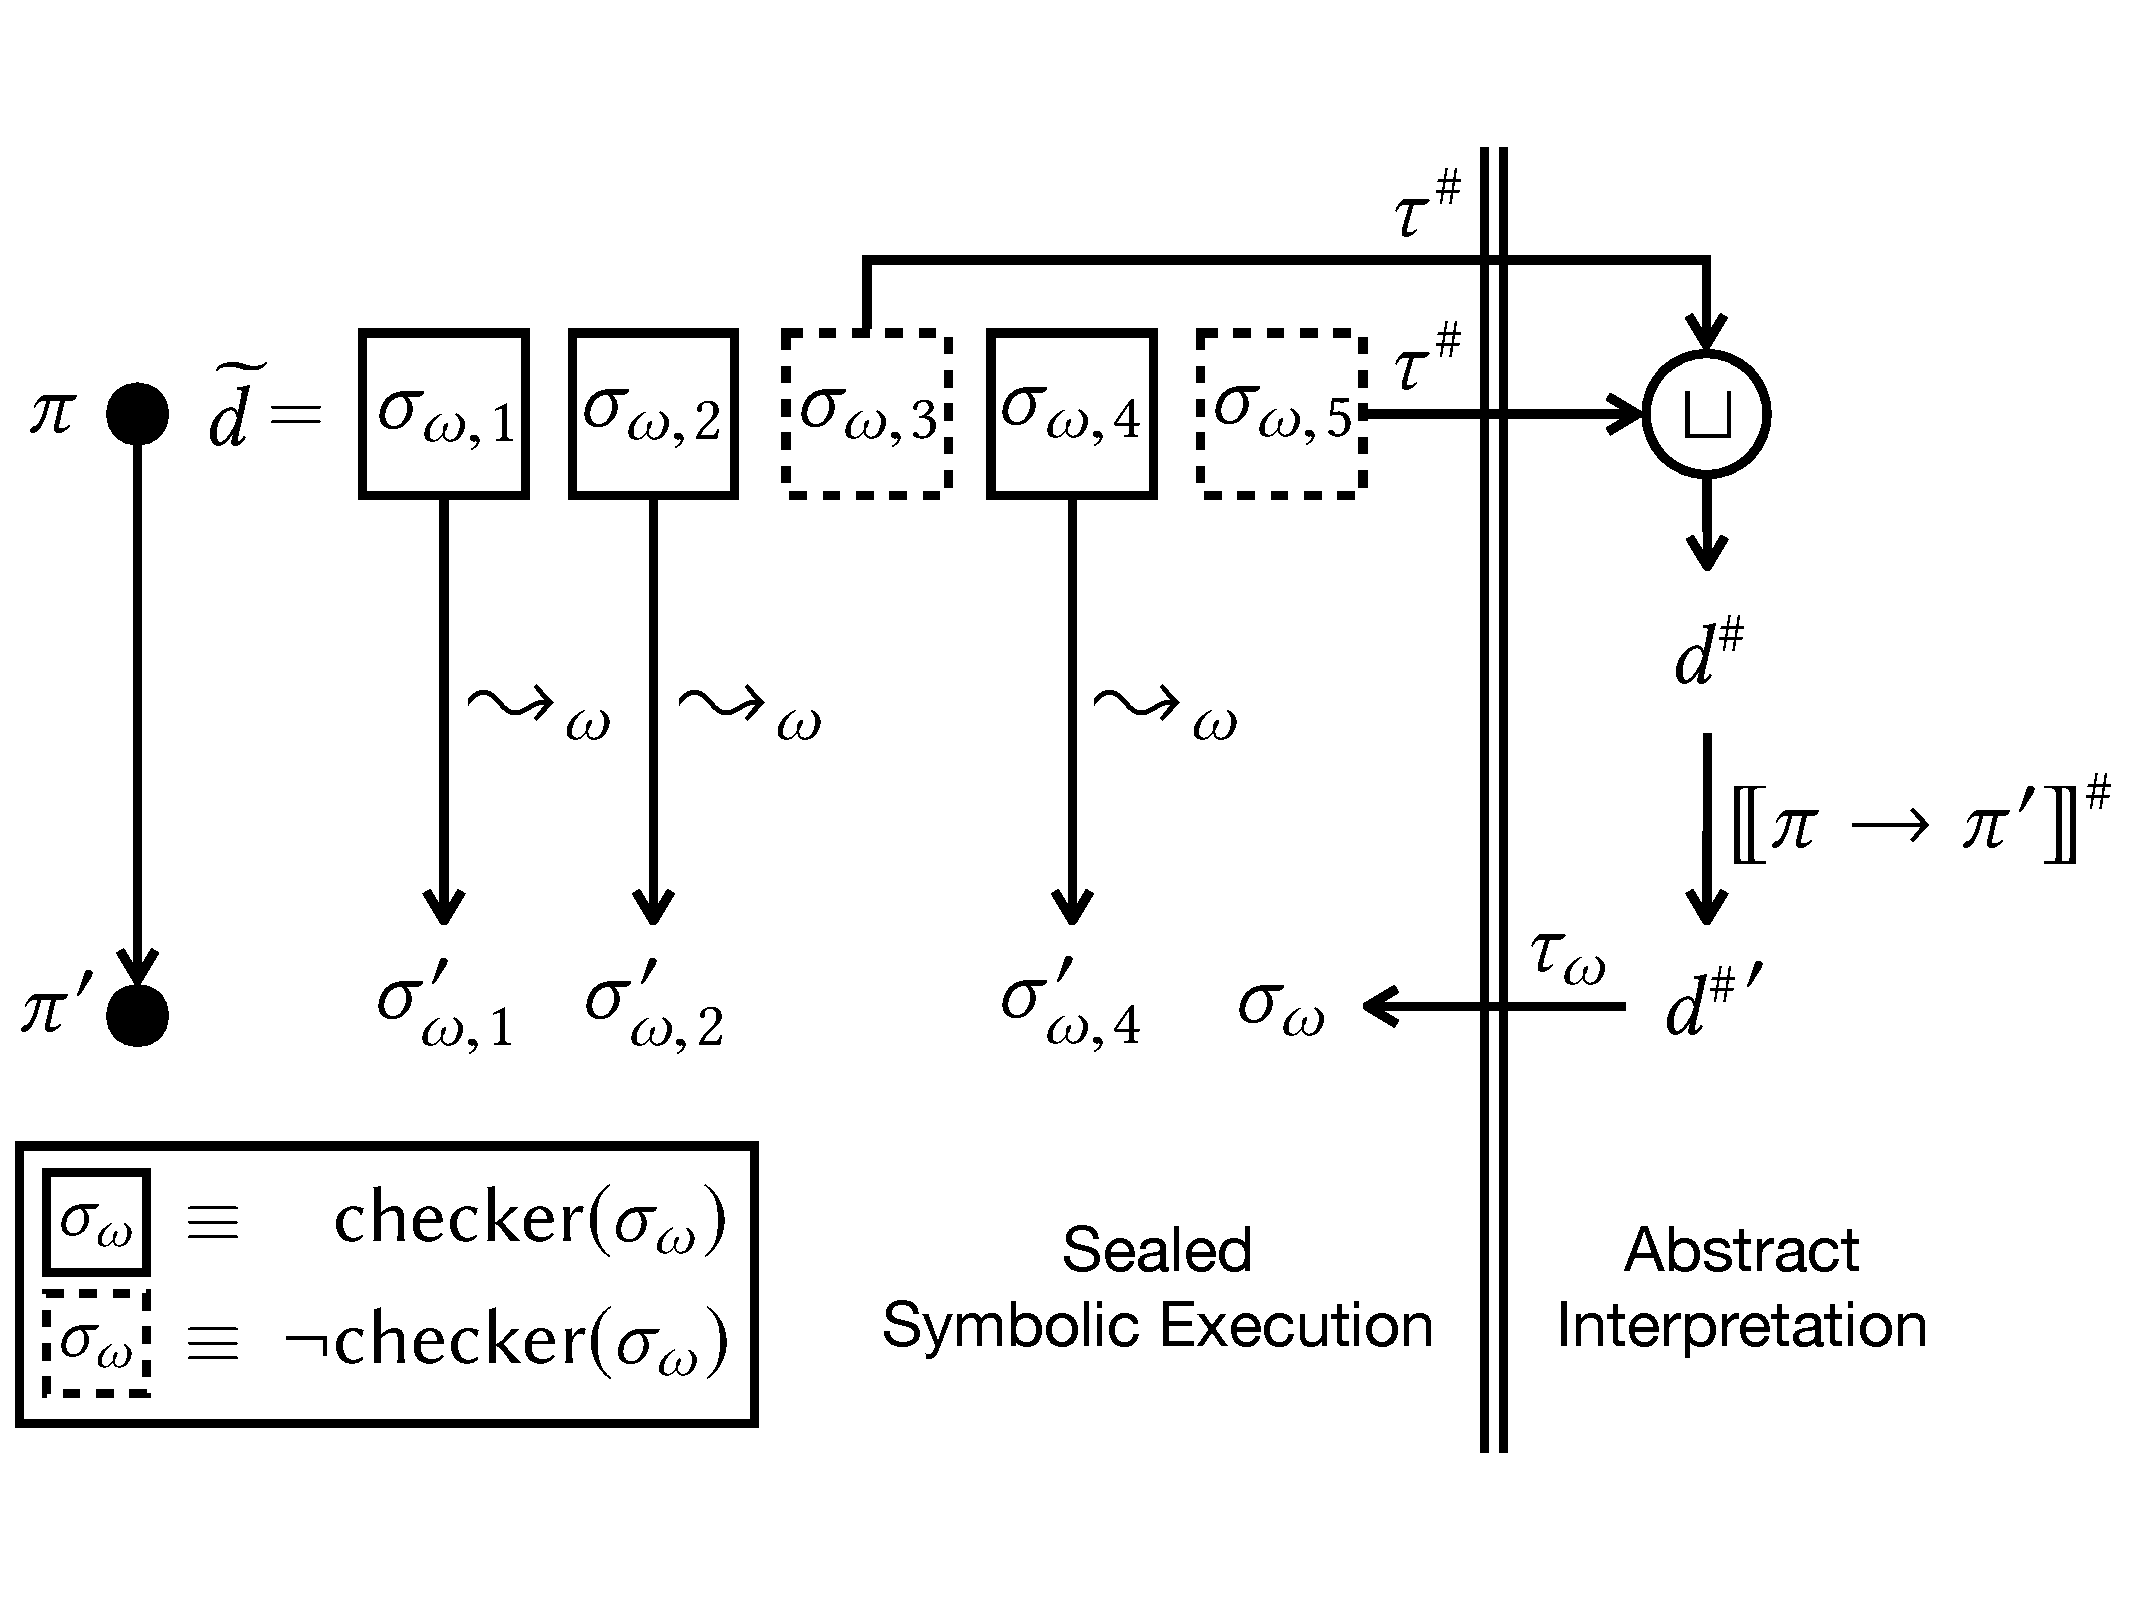
\includegraphics[width=\linewidth]{img/dynamic-shortcut}
  \vspace*{-2em}
  \caption{The diagram for the extended view transition for dynamic shortcut.}
  \vspace*{-1em}
  \label{fig:dynamic-shortcut}
\end{figure}

\begin{figure*}[t]
  \centering

  \fbox{$\st \trans \st$}
  \begin{mathpar}
    \inferrule*[width=0.48\textwidth]
    {
      \prog(\lab) = \refer = \expr\\
      \referrule{\st}{\refer}{\loc}\\
      \exprrule{\st}{\expr}{\val}\\
    }
    {
      \st = (\lab, \mem, \ctxt, \addr)
      \trans
      (\labnext(\lab), \mem[\loc \mapsto \val], \ctxt, \addr)
    }

    \inferrule*[width=0.48\textwidth]
    {
      \prog(\lab) = \refer = \kwobj\\
      \referrule{\st}{\refer}{\loc}\\
      \addr' = \text{(a fresh object address)}
    }
    {
      \st = (\lab, \mem, \ctxt, \addr)
      \trans
      (\labnext(\lab), \mem[\loc \mapsto \addr'], \ctxt, \addr)
    }

    \inferrule*[width=0.48\textwidth]
    {
      \prog(\lab) = \refer = \expr_f ( \expr_a )\\
      \referrule{\st}{\refer}{\loc}\\
      \exprrule{\st}{\expr_f}{\fval{x}{\lab_b}}\\
      \exprrule{\st}{\expr_a}{\val_a}\\
      \addr' = \text{(a fresh environment address)}
    }
    {
      \st = (\lab, \mem, \ctxt, \addr)
      \trans
      (\lab_b, \mem[(\addr', x) \mapsto \val_a], \ctxt[\addr' \mapsto (\addr,
      \labnext(\lab), \loc)], \addr')
    }

    \inferrule*[width=0.48\textwidth]
    {
      \prog(\lab) = \kwret \; \expr\\
      \exprrule{\st}{\expr}{\val}\\
      \ctxt(\addr) = (\addr', \lab', \loc)
    }
    {
      \st = (\lab, \mem, \ctxt, \addr)
      \trans
      (\lab', \mem[\loc \mapsto \val], \ctxt, \addr')
    }

    \inferrule*[width=0.48\textwidth]
    {
      \prog(\lab) = \kwif \; \expr \; \lab'\\
      \exprrule{\st}{\expr}{\kwtrue}\\
    }
    {
      \st = (\lab, \mem, \ctxt, \addr)
      \trans
      (\lab', \mem, \ctxt, \addr)
    }

    \inferrule*[width=0.48\textwidth]
    {
      \prog(\lab) = \kwif \; \expr \; \lab'\\
      \exprrule{\st}{\expr}{\kwfalse}\\
    }
    {
      \st = (\lab, \mem, \ctxt, \addr)
      \trans
      (\labnext(\lab), \mem, \ctxt, \addr)
    }
  \end{mathpar}

  \fbox{$\referrule{\st}{\refer}{\loc}$}
  \begin{mathpar}
    \inferrule*[width=0.48\textwidth]
    {}
    {
      \referrule{\st = (\lab, \mem, \ctxt, \addr)}{x}{(\addr, x)}\\
    }

    \inferrule*[width=0.48\textwidth]
    {
      \exprrule{\st}{\expr_0}{\addr_0}\\
      \exprrule{\st}{\expr_1}{\val_1}\\
      \val_1 \in \strset\\
    }
    {
      \referrule{\st = (\lab, \mem, \ctxt, \addr)}{\expr_0 [ \expr_1
      ]}{(\addr_0, \val_1)}
    }
  \end{mathpar}

  \fbox{$\exprrule{\st}{\expr}{\val}$}
  \begin{mathpar}
    \inferrule*[width=0.48\textwidth]
    {}
    {
      \exprrule{\st = (\lab, \mem, \ctxt, \addr)}{\pval}{\pval}
    }

    \inferrule*[width=0.48\textwidth]
    {}
    {
      \exprrule{\st = (\lab, \mem, \ctxt,
      \addr)}{\fval{x}{\lab'}}{\fval{x}{\lab'}}
    }

    \inferrule*[width=0.48\textwidth]
    {
      \referrule{\st}{\refer}{\loc}\\
      \loc \in \Dom(\mem)
    }
    {
      \exprrule{\st = (\lab, \mem, \ctxt, \addr)}{\refer}{\mem(\loc)}
    }

    \inferrule*[width=0.48\textwidth]
    {
      \exprrule{\st}{\expr_1}{\val_1}\\
      \cdots\\
      \exprrule{\st}{\expr_n}{\val_n}
    }
    {
      \exprrule{\st = (\lab, \mem, \ctxt, \addr)}
      {\op(\expr_1, \cdots, \expr_n)}{\op(\val_1, \cdots, \val_n)}
    }
  \end{mathpar}

  \caption{The transition relation for the core language of JavaScript}
  \label{fig:core-trans-rel}
\end{figure*}

We define the the abstract interpretation with \textit{dynamic shortcut}, which
is a concrete semantics on sealed symbolic execution.  With dynamic shortcut,
we use the powerset of symbolic states as the domain $\combdom =
\powerset{\symbstset}$, and extend the view transition as follows:
\[
  \begin{array}{l}
    \combviewtrans{\view}{\view'}(\combelem) =\\
    \qquad \{
      \symbst' \mid \symbst \in S \wedge
      \symbst \symbtrans \symbst' \wedge
      \saconverter(\symbst') = (\view', \_)
    \}\\
    \qquad \cup \left\{
    \begin{array}{ll}
      \{ \asconverter \circ \viewtrans{\view}{\view'}(\bigjoin D) \}
      & \text{if} \; D \neq \varnothing\\
      \varnothing & \text{otherwise}\\
    \end{array}
    \right.
  \end{array}
\]
where $S = \combelem\mid_{\checker}$ and $D =
\dot{\saconverter}(\combelem\mid_{\neg\checker})$.  The dot notation $\dot{f}$
denotes the element-wise extended function of a function $f$.  The abstract
interpretation with dynamic shortcut performs one-step symbolic transition for
each symbolic state that passes the filter $\checker$. On the other hand, it
converts remaining symbolic states to the corresponding abstract states, merges
them into a single abstract state, and performs the abstract one-step execution
for the abstract state.

For example, Figure~\ref{fig:dynamic-shortcut} depicts the
diagram of the extended view transition from $\view$ to $\view'$ for dynamic
shortcut.  The element $\combelem$ in $\view$ consists of five symbolic states
from $\nsymbst{1}$ to $\nsymbst{5}$.  The solid box denotes that the corresponding
symbolic state passes the filter $\checker$ and the dotted box denotes that it
does not.  For each symbolic state that passes the filter ($\nsymbst{1}$,
$\nsymbst{2}$, and $\nsymbst{4}$), it applies the symbolic transition $\symbtrans$.
For failed symbolic states ($\nsymbst{3}$ and $\nsymbst{5}$), it applies the
converter $\saconverter$ to convert each of them to the corresponding abstract
state and merges results using the join operator ($\join$).  Then, it utilizes
the abstract semantics via the original view transition
$\viewtrans{\view}{\view'}$ and the converter $\asconverter$ to convert the
result to the corresponding symbolic state.

We could configure when the sealed symbolic execution or the abstract
interpretation is performed based on the definition of the $\checker$ function
and its negation $\neg\checker$.  For example, we could define the $\checker$
that passes only function entry, call, and exit points to perform conversions in
a function level.  However, for the soundness and the termination of the
the abstract interpretation with dynamic shortcut, it should satisfy the
following condition:
\begin{theorem}\label{theorem:shortcut}
  The abstract interpretation with dynamic shortcut is sound and terminates in a
  finite time if its abstract semantics is sound and $\checker$ satisfies the
  following condition:
  \[
    \checker(\symbst) \Rightarrow \symbst \symbtrans^k \excst \wedge
    1 < k \leq N
  \]
  where $N$ is a pre-defined maximum length of the sealed symbolic execution.
\end{theorem}
\inred{We proved Theorem~\ref{theorem:shortcut} using the Kleene's fixed-point
theorem~\cite{kleene} with the finite height of abstract domains. Because of the
page limitation, we omit the proof in this paper and include it in a companion
report~\cite{report}.}
